\section{Training Optimization Strategies}

This section describes the training algorithms, learning rate schedules and regularization techniques used to improve model generalization and prevent overfitting.

\subsection{Training Algorithms and Optimizers}\label{subsec:training-algorithms-optimizers}

All models were trained using the Adam optimizer~\cite{kingma2017adammethodstochasticoptimization} with a learning rate of \textit{0.001}. The Adam optimizer is a popular choice for training deep neural networks due to its adaptive learning rate mechanism and momentum-based updates. A weight decay of \textit{1e-4} was applied to regularize the model and prevent overfitting~(see~\ref{subsec:regularization-techniques}).

\subsection{Learning Rate Schedules}

To adjust the learning rate during training, a learning rate scheduler was used to reduce the learning rate by a factor of \textit{0.5} if the validation loss did not improve for \textit{2} epochs. This technique helps the model converge more effectively by gradually reducing the learning rate as it approaches a local minimum.

\subsection{Regularization Techniques}\label{subsec:regularization-techniques}

To prevent overfitting and improve generalization, several regularization techniques were applied during training:

\begin{itemize}
    \item \textbf{Weight Decay:} L2 regularization with a weight decay of \textit{1e-4} was applied to the optimizer to penalize large weights (see~\ref{subsec:training-algorithms-optimizers}).
    \item \textbf{Dropout:} A dropout layer with a dropout probability of \textit{0.5} was added after the fully connected layer to regularize the model and prevent co-adaptation of neurons.
    \item \textbf{Data Augmentation:} Various data augmentation techniques such as random rotations, flips and color jittering were applied to the training images to increase the diversity of the training set and improve the robustness of the model~(see Fig.~\ref{fig:data-augmentation}).
\end{itemize}

\begin{figure}[htbp]
    \centerline{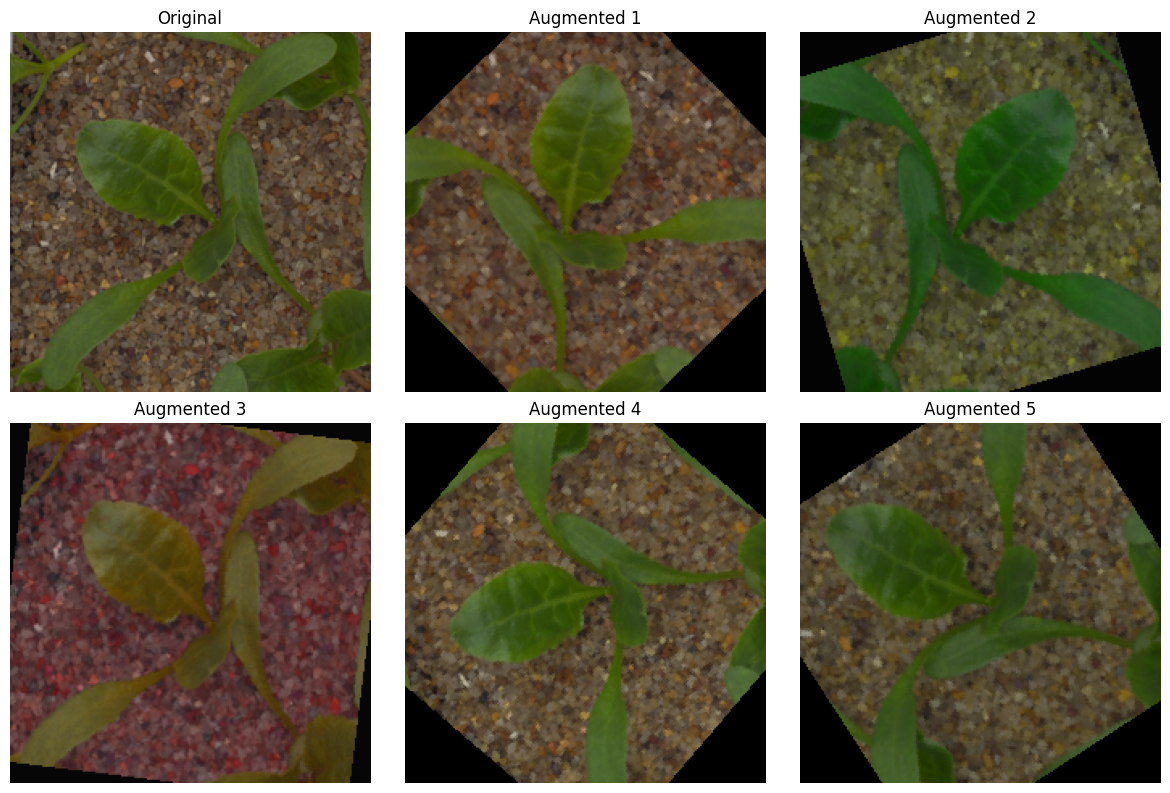
\includegraphics[width=0.9\linewidth]{../../resources/data_augmentation.png}}
    \caption{Original image~(top left) and five augmented versions.}
    \label{fig:data-augmentation}
\end{figure}

Fig.~\ref{fig:data-augmentation} shows one original image of the given dataset and five augmented versions. The augmentations include random rotations, flips and color jittering, which help the models learn more robust features and improve generalization to unseen data. During training those augmentations were applied randomly to each image, while the original images were used for validation. This approach allowed the model to learn from a more diverse set of training samples without introducing bias in the validation process.